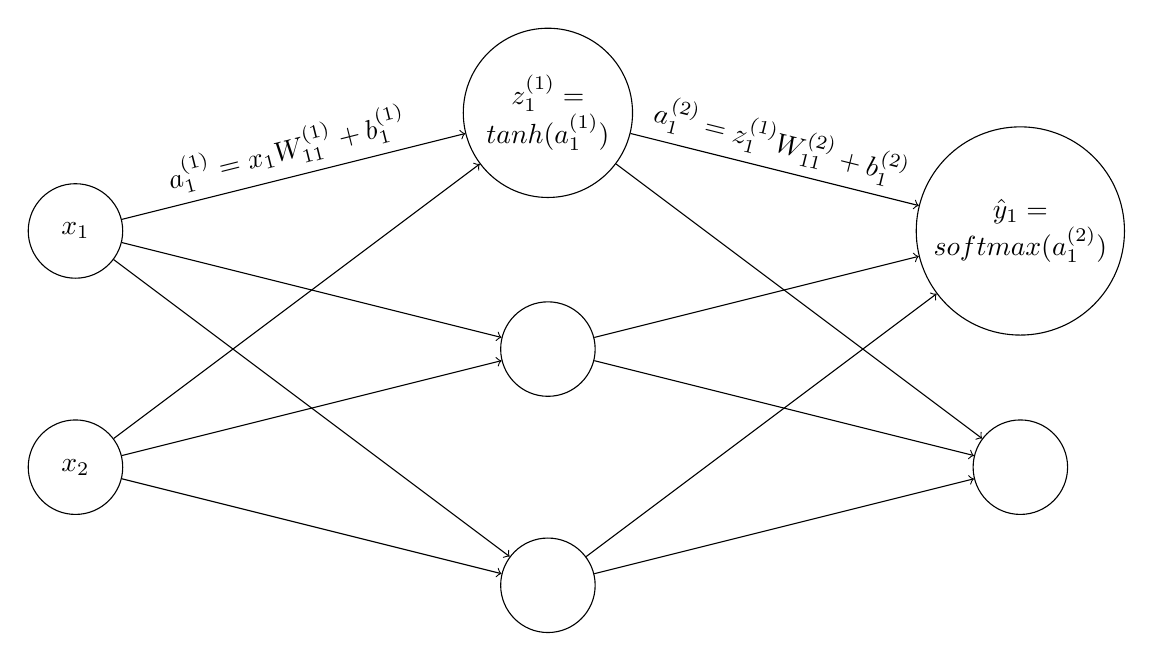
\begin{tikzpicture}
\centering
\node at (0,0) {  };
\node at (0,6.66667) {  };
\node at (12,6.66667) {  };
\node at (12,0) {  };
\node[draw,circle,minimum size=1.2cm,name=n00,align=center] at (0,1.83333) {$x_2$};
\node[draw,circle,minimum size=1.2cm,name=n01,align=center] at (0,4.83333) {$x_1$};
\node[draw,circle,minimum size=1.2cm,name=n10] at (6,0.333333) {};
\node[draw,circle,minimum size=1.2cm,name=n11] at (6,3.33333) {};
\node[draw,circle,minimum size=1.2cm,name=n12,align=center] at (6,6.33333) {$z_{1}^{(1)} =$\\$ \text{tanh}(a_{1}^{(1)})$};
\node[draw,circle,minimum size=1.2cm,name=n20] at (12,1.83333) {};
\node[draw,circle,minimum size=1.2cm,name=n21,align=center] at (12,4.83333) {$\hat{y}_{1} =$\\$ \text{softmax}(a_{1}^{(2)})$};
\draw[->,name=a0010] (n00) -- (n10);
\draw[->,name=a0011] (n00) -- (n11);
\draw[->,name=a0012] (n00) -- (n12);
\draw[->,name=a0110] (n01) -- (n10);
\draw[->,name=a0111] (n01) -- (n11);
\draw[->,name=a0112] (n01) -- node[sloped,anchor=center,above] {$a_{1}^{(1)} =x_{1}W_{11}^{(1)} + b_1^{(1)}$} (n12);
\draw[->,name=a1020] (n10) -- (n20);
\draw[->,name=a1021] (n10) -- (n21);
\draw[->,name=a1120] (n11) -- (n20);
\draw[->,name=a1121] (n11) -- (n21);
\draw[->,name=a1220] (n12) -- (n20);
\draw[->,name=a1221] (n12) -- node[sloped,anchor=center,above] {$a_{1}^{(2)} =z_{1}^{(1)}W_{11}^{(2)} + b_1^{(2)}$} (n21);
\end{tikzpicture}
